\section{Methodology}
\label{Methodology}
% \setcounter{equation}{0}

\subsection{Introduction to Methodology}

In this section, we first introduce ML, and its learning paradigms such as supervised learning (SL), unsupervised learning (UL), and reinforcement learning (RL). We discuss our research questions in the context of a classification problem using SL. Then, we introduce the models used in this thesis, namely logistic regression using GLM, and XGBoost. Next, we introduce metrics used to assess model performance in \autoref{Results and discussion}. We introduce the confusion matrix and derived metrics, such as accuracy, precision, sensitivity, specificity, and F-score. We also describe descriptive plots as area under operating characteristic curve (AUROC) and variable importance plots (VIP).

\subsection{Machine Learning}

\textcite{samuel-some-studies-in-machine-learning-using-the-game-of-checkers} is accredited with introducing the term ML. He states that ML is a field of study that makes computers learn without explicitly being programmed \parencite{samuel-some-studies-in-machine-learning-using-the-game-of-checkers}. ML described the pattern recognition tasks from the learning component of artificial intelligence (AI), which in itself was introduced by \textcite{mccarthy-artificial-intelligence}. \textcite{samuel-some-studies-in-machine-learning-using-the-game-of-checkers} applied ML to the game of checkers, a game having clear rules and motivations. Following breakthroughs in ML \parencite{sutskever-neural-network}, and AI during the last decade \parencite{vaswani-attention-is-all-you-need}, the world has experienced massive increases in the application of ML. This is especially shown through tools such as large language models \parencite{open-ai-gpt-4}.

\textcite{ban404-the-elements-of-statistical-learning} describe ML as a set of methods for identifying patterns and trends in large data sets. This is expanded by \textcite{ban404-an-introduction-to-statistical-learning}, who discusses statistical learning as a tool for interpreting complex data. ML is mainly divided into SL, UL, and RL \parencite{ban404-an-introduction-to-statistical-learning}. SL focuses on predicting an output variable from input variables, while UL aims to uncover patterns and associations among input variables without a specific output variable \parencite{ban404-the-elements-of-statistical-learning}. In RL, one trains an ML model to move towards something, refining its behaviour through cost functions \parencite{sutton-reinforcement-learning}. The three types of ML all have useful applications in different contexts \parencite{ban404-the-elements-of-statistical-learning}. In this thesis, we apply SL when predicting index composition on OSEBX.

\textcite{white-ibm-neural-networks} made an early application of ML in finance, forecasting the daily stock returns of the US company IBM. The following decades experienced massive increases in the application of ML in finance \parencite{warin-machine-learning-in-finance-metadata}. \textcite{goodell-artificial-intelligence-and-machine-learning-in-finance} divides current themes of ML in finance into (1) portfolio construction, (2) financial fraud, and (3) forecasting. In our context, trading on predicted upcoming additions and deletions using ML fits the first theme \parencite{goodell-artificial-intelligence-and-machine-learning-in-finance}.  

\subsection{Logistic Regression}

Regression analysis is a statistical method for predicting a dependent variable based on one or more independent variables, often used to determine relationships and trends \parencite{galton-regression}. \textcite{cox-the-regression-analysis-of-binary-sequences} furthered the concept to binary sequences, classifying outcomes as success/failure, or 1/0. This concept forms the basis of classification problems \parencite{cox-the-regression-analysis-of-binary-sequences}. Using ML to assign new input vectors of explained variables to a finite number of target categories is named a classification problem \parencite{bishop-pattern-recognition-and-machine-learning}. If the target output is comprised of continuous variables, this is a regression problem \parencite{bishop-pattern-recognition-and-machine-learning}.  

Regression presupposes ordered relationships between outcomes, such that ordinary least squares (OLS) can be used to fit a model \parencite{ban404-the-elements-of-statistical-learning}. This approach does not make sense when predicting classes, which do not have such linearly ordered relationships \parencite{ban404-the-elements-of-statistical-learning}. Linear models are suitable for regression \parencite{pearson-linear-regression}, but struggle with the binary nature of a classification problem. Logistic regression uses a logistic function to ensure outputs between 0 and 1, representing probabilities \parencite{berkson-logistic-regression}. This makes it ideal for classification tasks where outcomes are distinctly categorical \parencite{berkson-logistic-regression}. 

In logistic regression, a linear combination of independent variables represented as $z$ with coefficients $\beta_0$ and $\beta_1$ in \autoref{equation:logit-linear-combination}, is transformed by the logistic function into a probability. This maps the linear combination to a value in the interval [0,1], as in \autoref{equation:logit-applying-linear-combination}. Combining these steps, the logistic regression model is fully expressed in \autoref{equation:logit-expanded-regression-model}. 

\begin{equation}
\label{equation:logit-linear-combination}
    z = \beta_0 + \beta_1X
\end{equation}
\begin{equation} 
\label{equation:logit-applying-linear-combination}
    p(X) = \frac{1}{1 + e^{-z}}
\end{equation}
\begin{equation} 
\label{equation:logit-expanded-regression-model}
    p(X) = \frac{e^{\beta_0 + \beta_1X}}{1 + e^{\beta_0 + \beta_1X}}
\end{equation}

\textcite{glm-generalized-linear-models} introduced GLM, which enhances traditional linear models by using iterative weighted regression for efficient parameter estimation via maximum likelihood. We apply logistic regression using GLM in R (as our main analytical tool), with the function \texttt{glm::glm()} \parencite{glm-r-documentation}. In R, \texttt{y} is the target variable, \texttt{x} the predictor variables, \texttt{family=binomial} the binomial distribution, and \texttt{link="logit"} specifying the use of logistic regression.

\subsection{Tree Boosting Models}

\textcite{schapire-the-strength-of-weak-learners} first introduced the procedure for boosting models. Boosting models build on an initial model, and use base models to \textit{boost} accuracy over sequential iterations. He showed that weak learners could improve their model performance when training additional classifiers \parencite{schapire-the-strength-of-weak-learners}. In this context, a weak learner is an algorithm for producing a two-class classifier that outperforms random chance. The weak learner algorithm improves on an initial classifier $h_1$ by \textit{boosting} model performance over several iterations. \textcite{schapire-the-strength-of-weak-learners} was first able to prove that the boosted classifier $h_B$ outperform the initial $h_1$ in model performance. In \autoref{schapire-algo}, \textcite{friedman-additive-logistic-regression} illustrate the boosting algorithm by \textcite{schapire-the-strength-of-weak-learners}. 

\begin{algorithm}[H]
\caption{Schapire Weak Learner Algorithm \parencite{friedman-additive-logistic-regression}}
\label{schapire-algo}
\begin{algorithmic}[1]
\Statex \textbf{Input:} Data training set $D$, number of data points $N$.
\State $h_1$ is learned on first $N$ training points in $D$;
\State $h_2$ is learned on a new sample of $N$ point in $D$, where half are misclassified by $h_1$;
\State $h_3$ is learned on $N$ points in $D$, where $h_1$ and $h_2$ disagree
\State $h_B$ is the boosted classifier, where $h_B = \text{Majority Vote}(h_1,h_2,h_3)$
\Statex \textbf{Output:} Boosted classifier $h_B$
\end{algorithmic}
\end{algorithm}

Tree boosting has proven to be a highly efficient ML model in doing predictions \parencite{xgboost-a-scaleable-tree-boosting-system}. Tree boosting builds on intuition by \textcite{schapire-the-strength-of-weak-learners}. Both the base learner and base models are simple. In other words, they typically have high bias and low variance \parencite{ntnu-thesis-why-does-xgboost-win-every-machine-learning-competition}. Tree boosting start with an initial model and find the final model by iterating $M$ times over base models. For each iteration $m$ where $m=1,\dots,M$, tree boosting models seek to minimise a loss function compared to the true target variable in the training data set. Each base model is weighted, which shows their contribution to the final model \parencite{ntnu-thesis-why-does-xgboost-win-every-machine-learning-competition}. 

In this context, a base model can be a simple decision tree model. Tree boosting is somewhat backward compared to classical ML algorithms, as the base models are evaluated compared to the true value of the target variable in training. As such, one could expect tree boosting to produce biased models. There is commonly a trade-off between bias and variance in a model \parencite{briscoe-bias-variance-tradeoff}, which is illustrated in \autoref{figure:bias-variance}. Tree boosting alleviate this by iterating for large values of $M$, penalising complex models, and scaling down base models by learning rates (or shrinkage).

\begin{figure}[H]
    \centering
    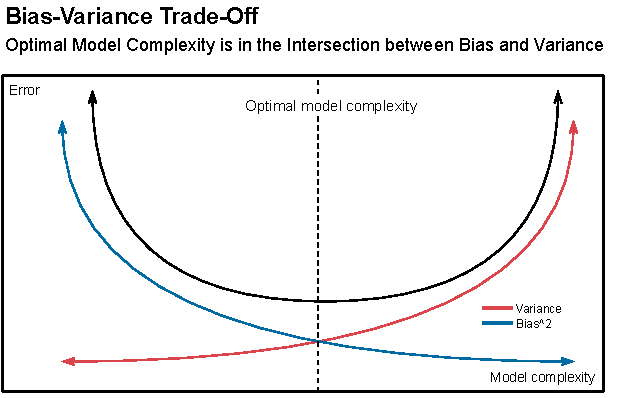
\includegraphics[width=0.8\textwidth]{images/bias-variance.drawio (2).pdf}
    \vspace{1em}
    \caption{{Bias-Variance Trade-Off}}
    \subcaption*{The model complexity is in a trade-off between bias and variance. Here, over-fitting typically entails high bias and low variance, while under-fitting entails low bias and high variance.}
    \label{figure:bias-variance}
\end{figure}

There exist other tree models which can improve the performance of a simple decision tree. Random forest (RF) is one such example, where a "forest" of many decision trees are generated. Here, the prediction made by the final RF model is the average prediction across a single iteration of a single forest. In \autoref{from-decision-tree-to-xgboost} we illustrate a single decision tree model and show the difference between a RF and tree boosting model. Typically, the performance ordering of these are single tree model $<$ RF $<$ tree boosting \parencite{ban404-an-introduction-to-statistical-learning}.  

\begin{figure}[H]
    \centering
    \vspace{1em}
    \begin{subfigure}{0.3\linewidth}
        \centering
        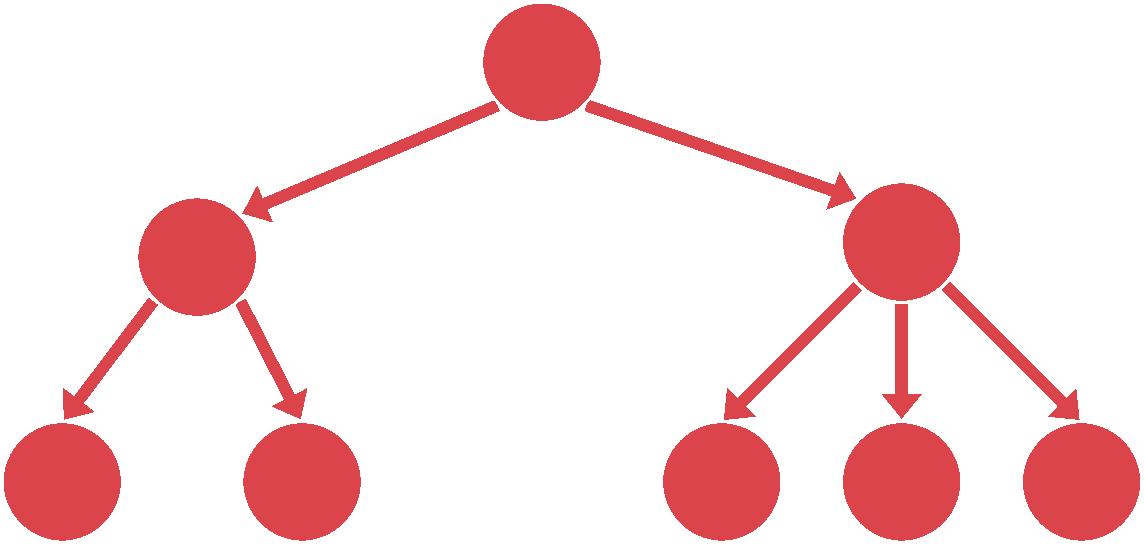
\includegraphics[width=\linewidth, height=\linewidth, keepaspectratio]{images/tree models.drawio.pdf}
        \caption{}
        \label{fig:draw-io-decision-tree}
    \end{subfigure}
    \hfill
    \begin{subfigure}{0.3\linewidth}
        \centering
        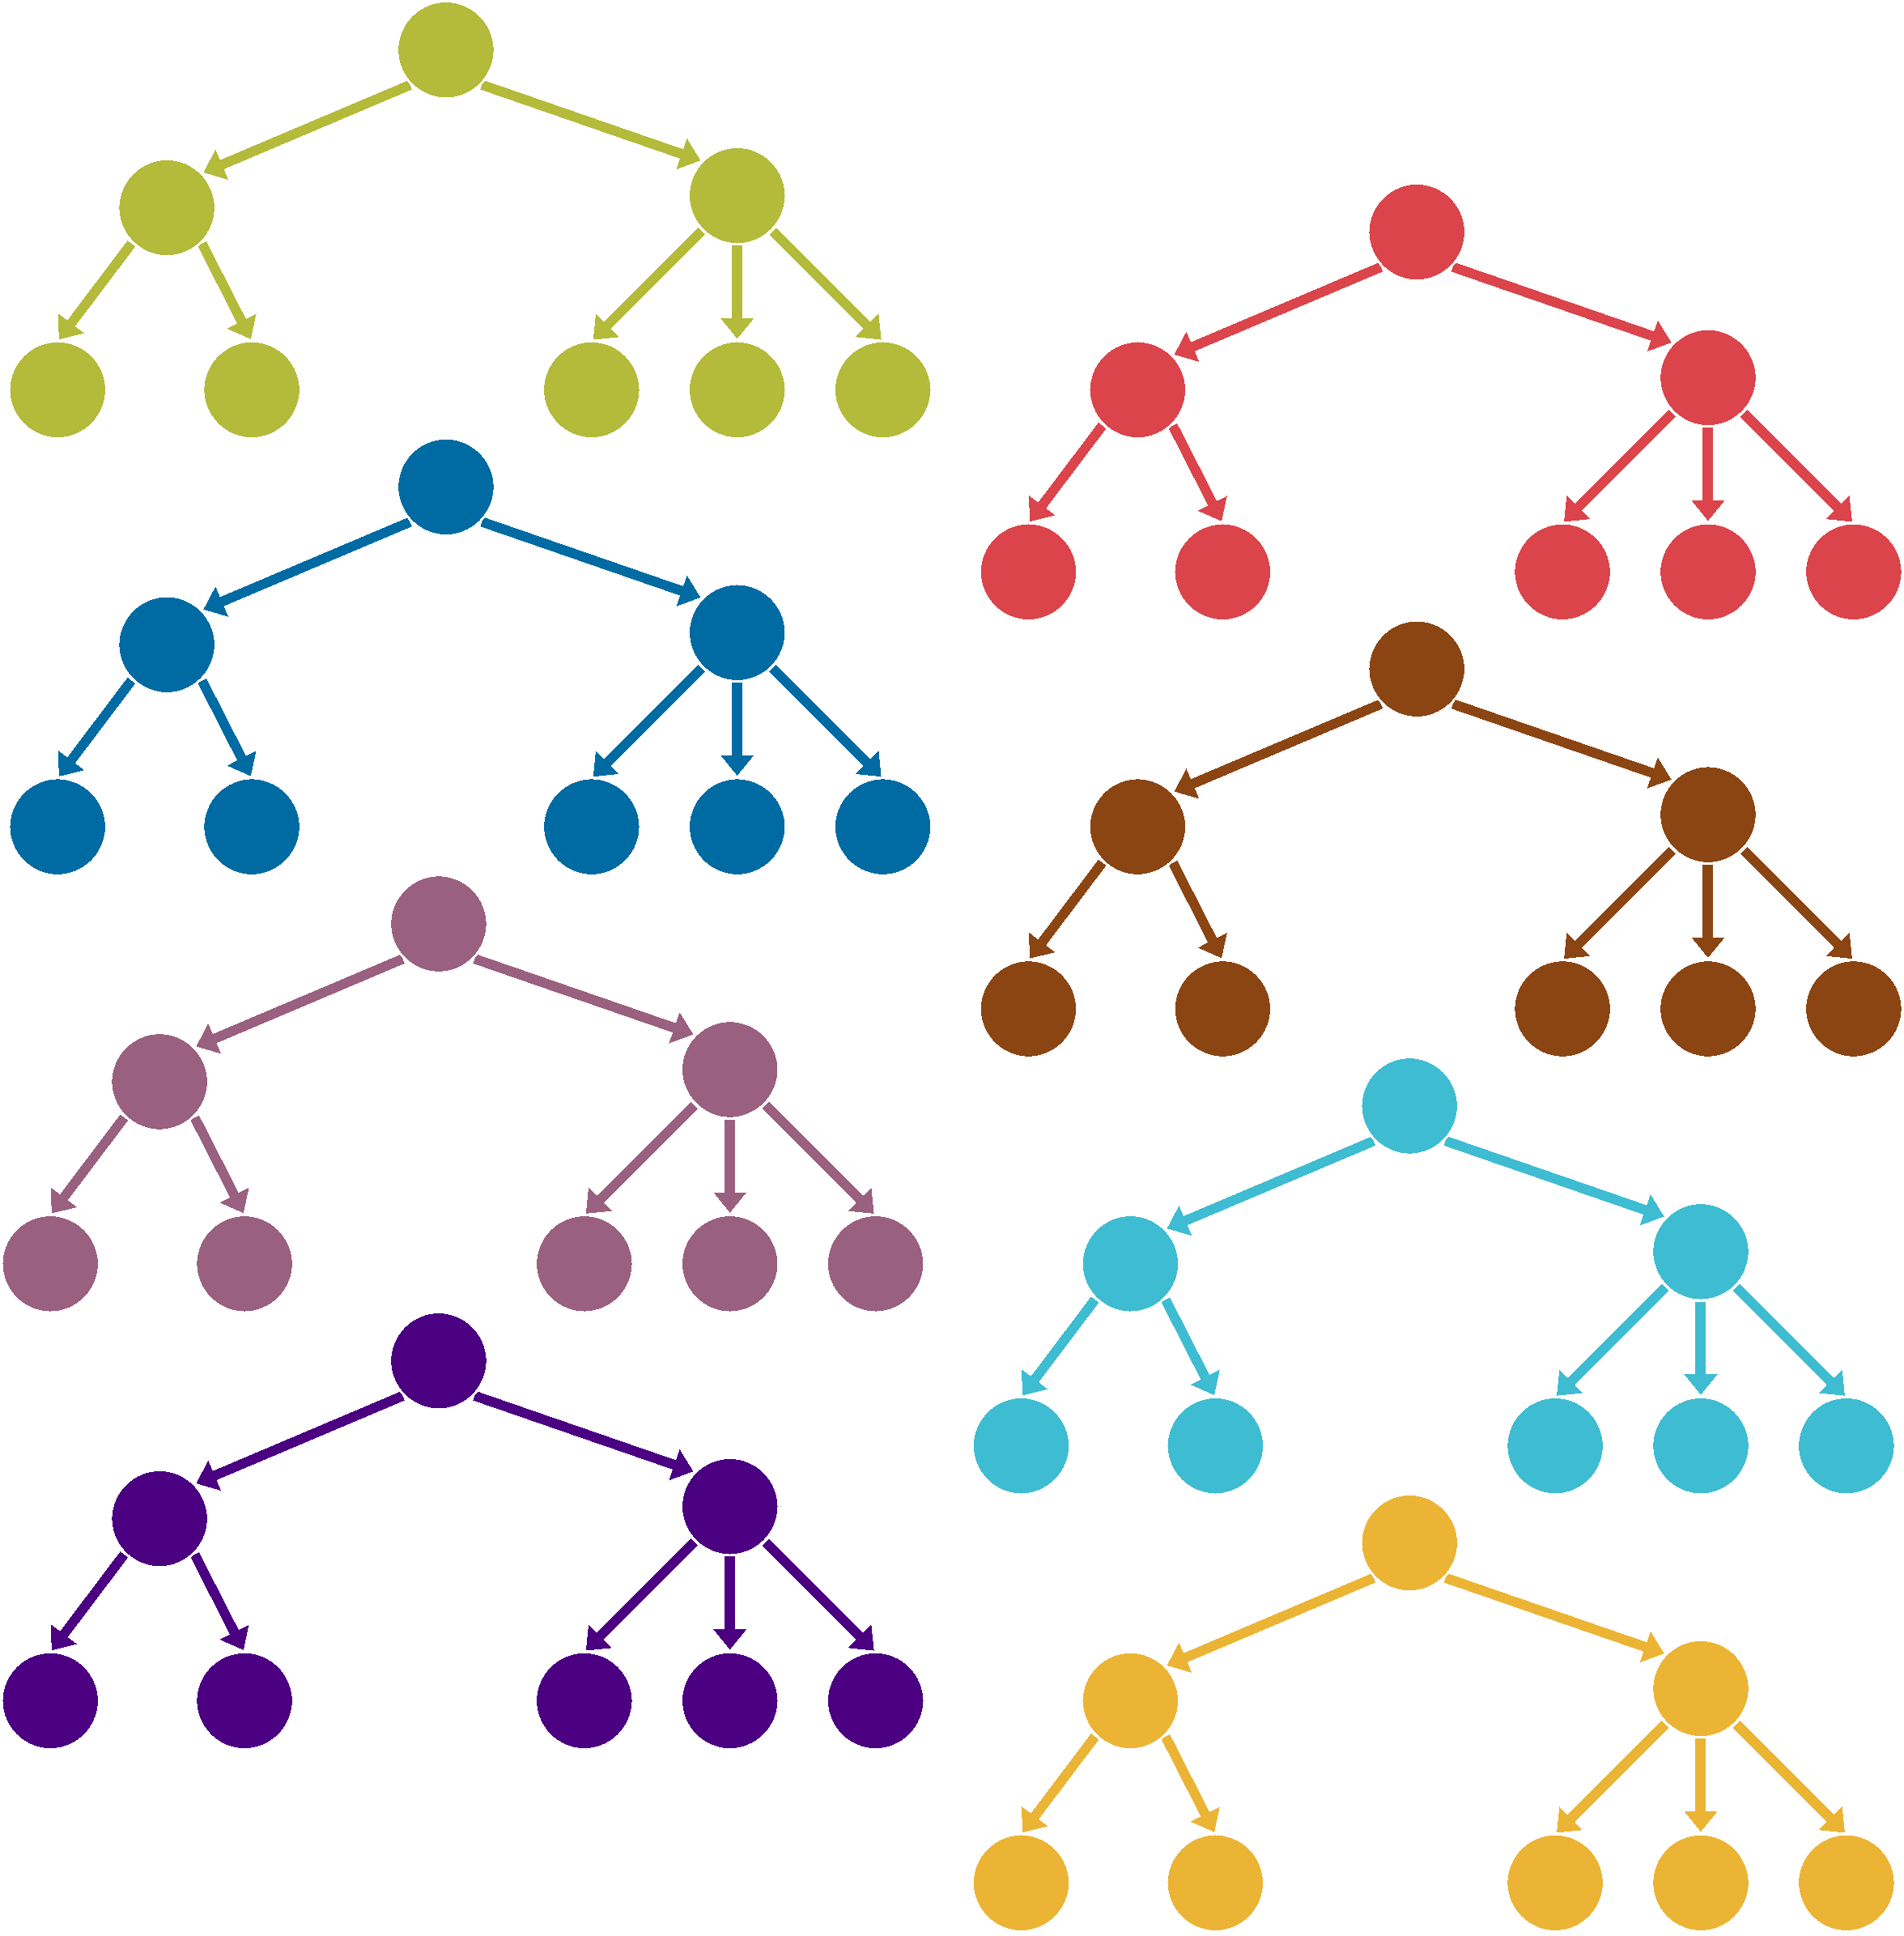
\includegraphics[width=\linewidth, height=\linewidth, keepaspectratio]{images/random forest diagram.drawio.pdf}
        \caption{}
        \label{fig:draw-io-random-forest}
    \end{subfigure}
    \hfill
    \begin{subfigure}{0.3\linewidth}
        \centering
        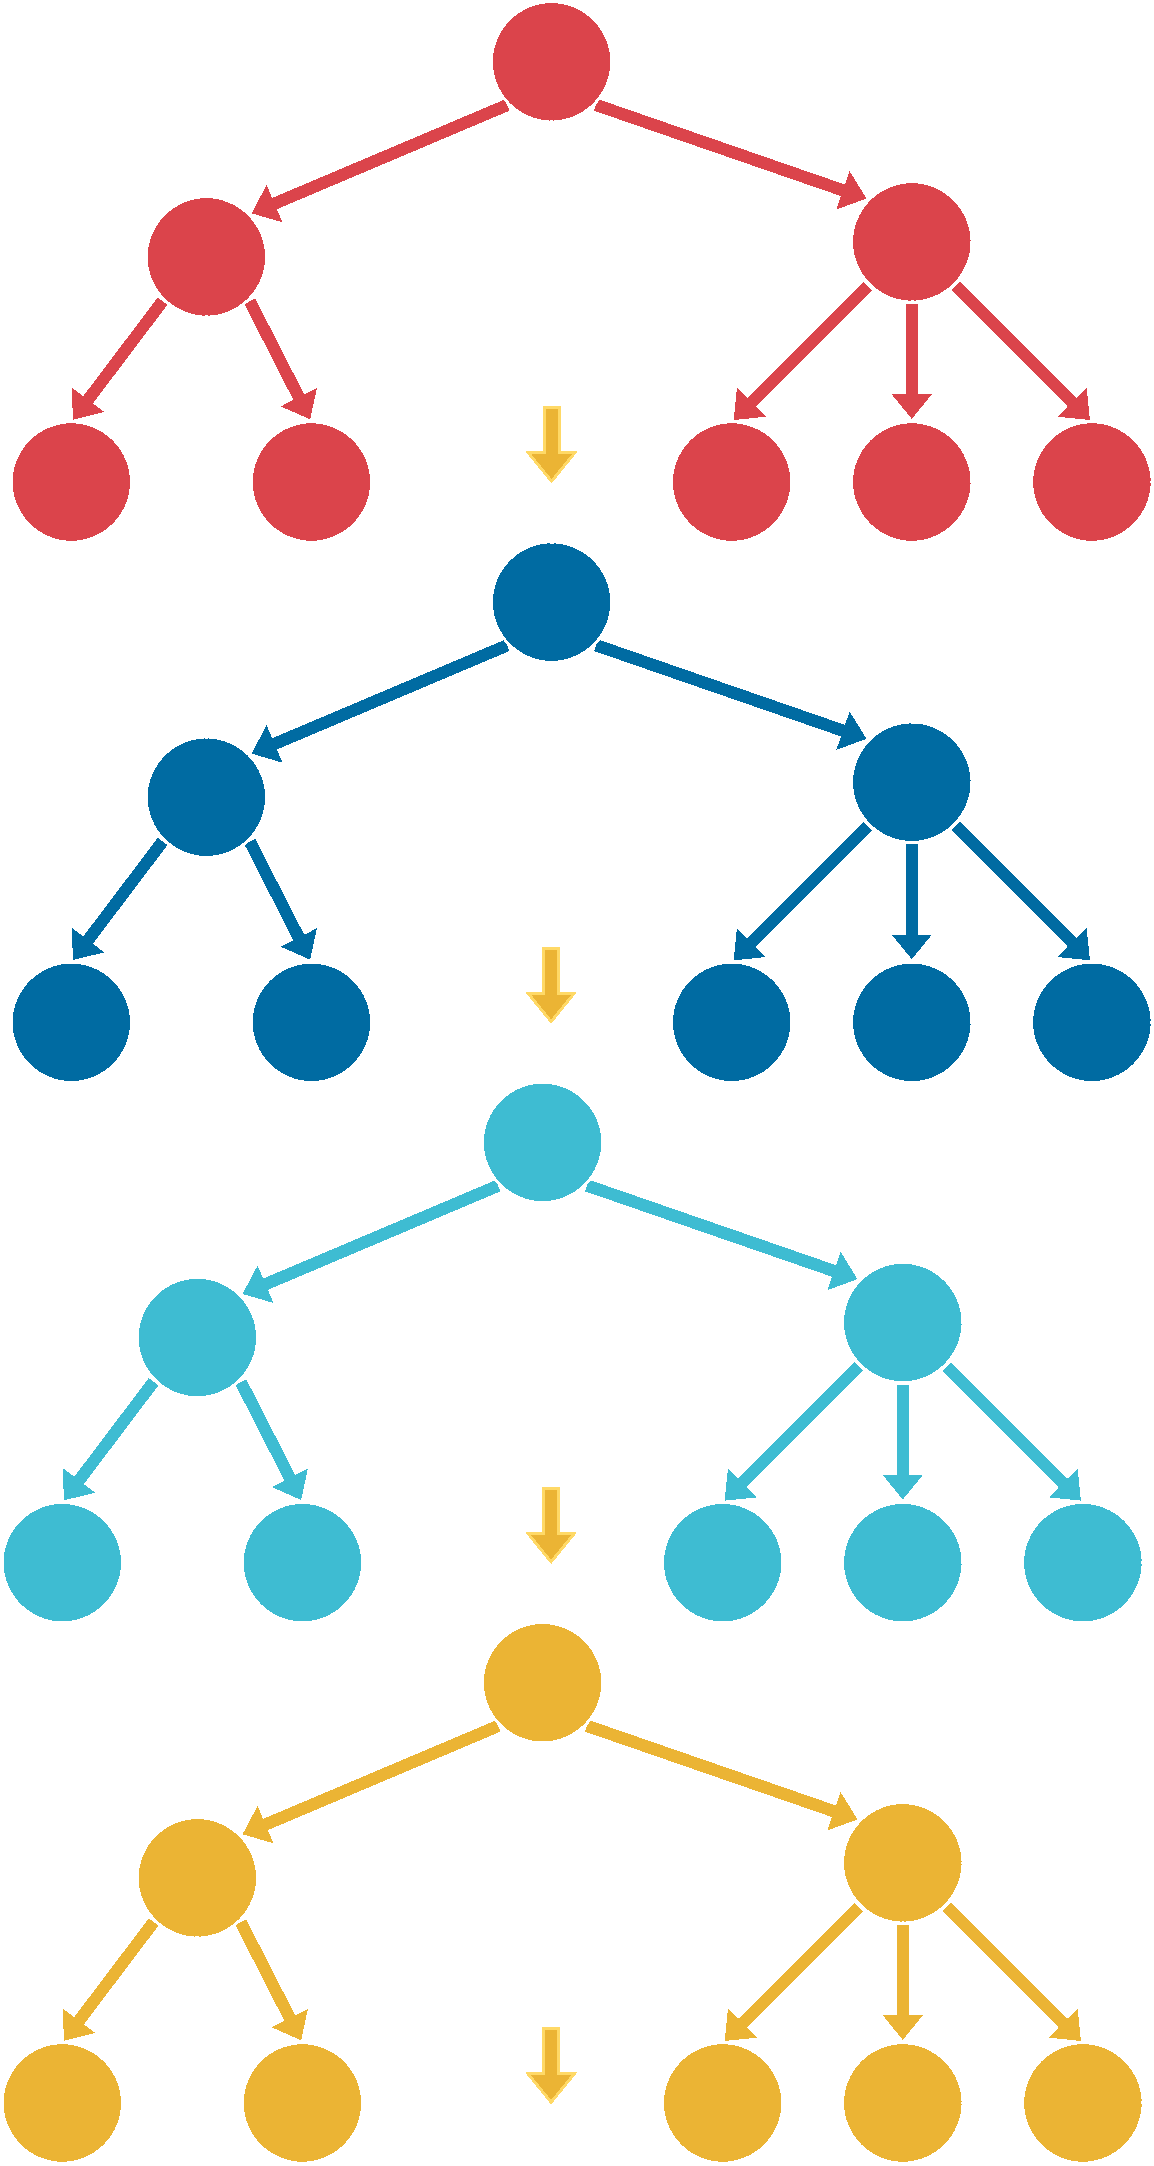
\includegraphics[width=\linewidth, height=\linewidth, keepaspectratio]{images/xgb.drawio.pdf}
        \caption{}
        \label{fig:draw-io-xgboost}
    \end{subfigure}
    \vspace{1em}
    \caption{{From a Single Tree Model (a) to Random Forest (b) to Tree Boosting (c)}}
    \subcaption*{We illustrate the simple intuition behind going from a single decision tree toward more complex tree models. RF average across a single iteration of several trees, while tree boosting aggregate over several iterations of a single tree.}
    \label{from-decision-tree-to-xgboost}
\end{figure}

\subsection{XGBoost}

Following tree-boosting algorithms producing competitive and robust classification models, \textcite{friedman-greedy-function-approximation} introduced gradient boosting. This is based on gradient descent. In other words, gradient boosting seeks to optimise an algorithm by finding the minimum of a function. It does so by moving opposite to the gradient of the function, or steepest ascent. The move from gradient to hessian boosting includes using not only first-order (gradient), but also second-order (hessian) methods when optimising boosting algorithms \parencite{ntnu-thesis-why-does-xgboost-win-every-machine-learning-competition}. XGBoost by \textcite{xgboost-a-scaleable-tree-boosting-system} is a tree boosting model which utilise both gradient and hessian boosting.  

The last years have seen a prominent rise in the popularity of XGBoost, by winning several ML competitions \parencite{ntnu-thesis-why-does-xgboost-win-every-machine-learning-competition}. XGBoost is renowned for its efficiency and flexibility in handling various data types, and the ability to customise XGBoost has made it an optimal tree-boosting system of choice in ML competitions \parencite{ntnu-thesis-why-does-xgboost-win-every-machine-learning-competition}. 

The function \texttt{xgboost::xgboost()} is an application of this in R \parencite{xgboost-package-yuan}. The documentation builds on work by \textcite{friedman-additive-logistic-regression} and \parencite*{friedman-greedy-function-approximation}. XGBoost comes with a wide range of configurable hyperparameters, which can be used to utilise the full potential of the model \parencite{kaggle-xgboost-hyperparameter}. The hyperparameters might be optimised to increase a specific measure, but in our application, we have used a set of parameters without optimising. This is mainly due to the low complexity of our classification problem. Hyperparameters used in this thesis are shown in \autoref{xgb-hyperparameters}.


\subsection{Posterior Probability Threshold}

The ML models output an estimated likelihood of which class the observations belong to, but the actual classification is determined based on the likelihood being above or below a certain threshold. This threshold is often set to 0.5, but in some practical applications, the predictions can be improved by using a different threshold \parencite{ban404-an-introduction-to-statistical-learning}. As \textcite{ban404-an-introduction-to-statistical-learning} mentions, when predicting if a bank customer is going to default or not, one can adjust the threshold to increase accuracy. \textcite{ban404-an-introduction-to-statistical-learning} refer to this threshold as the \textit{posterior probability threshold} (\textit{PPT}). In short, PPT can be adjusted to accommodate for specific use cases and increase accuracy. In this thesis, PPT can influence the distribution of the predicted additions and deletions to OSEBX, and also the total accuracy. In \autoref{Results and discussion}, we carefully consider which PPT should be applied in this thesis.

\subsubsection{Conditional Posterior Probability Threshold}

In our classification problem, it becomes evident that it is difficult for the ML algorithms to capture when a company is added or deleted from OSEBX. This is a practical challenge because we are dependent on predicting additions and deletions to exploit the index effect. We have considered several approaches to cope with this difficulty. First, we considered (1) implementing a custom objective function in the XGBoost application programming interface (API), where XGBoost enables for customising a loss function and a corresponding evaluation measure. The idea here would be to create a custom objective function to penalise model behaviour when not predicting changes. A different approach is to (2) implement a \textit{conditional PPT}, based on the status of the company in the previous period. The second approach considered is fairly easy to implement, and we investigate this approach further.

Seeking to increase the number of predicted changes made by the ML model, we add a lower PPT for companies not currently on the index (potential predicted additions), and a higher PPT for companies currently on the index (potential predicted deletions). To apply this in practice, let $Y_{i,t}$ represent the class for company $i$ at time $t$. Then $Y_{i,t-1}$ represents the class for company $i$ in the previous period $t-1$. By knowing the $Y_{i,t-1}$ for a specific observation, we can use this information to decide which PPT we would like to apply for that specific classification. When $Y_{i,t-1}$ is equal to 1, we know that the company was listed on OSEBX in the previous period. To increase the total number of predicted deletions, we would therefore use a higher PPT for this classification. In contrast, if $Y_{i,t-1}$ is equal to 0, we would like to lower the PPT, because then we would predict more additions to OSEBX. Next, we introduce a parameter $\varepsilon$ which is either added or subtracted from the PPT. We also define $\theta$ as the PPT, and $\theta^\star$ to be the conditional PPT. The conditional PPT can then be expressed as in \autoref{postprocessing}. 

\vspace{-1em}
\begin{equation}
\begin{aligned}
    \theta^\star = \begin{cases}
    \theta + \varepsilon, &  Y_{i, t-1} = 1 \\
    \theta - \varepsilon, &  Y_{i, t-1} = 0
    \end{cases}
\label{postprocessing}
\end{aligned}
\end{equation}

By using this equation, we must also define the valid values for $\theta^\star$, which can be expressed as $0 < \theta^\star < 1$. When classifying the observations, the predicted class $\widehat Y_{i,t}$ is 1 if the estimated probability $p$ is greater than $\theta^\star$, and 0 if $p$ is smaller than $\theta^\star$. To interpret \autoref{postprocessing} in words, we can describe it as the following: To keep staying on OSEBX will require a higher estimated probability, than entering OSEBX will require. Vice versa, to keep staying off OSEBX will require a lower estimated probability, than exiting OSEBX will require. 

However, by using this approach, we encounter some important considerations. First, if a higher number of trades is better at capturing the index effect, why not buy all companies currently not on OSEBX, and sell all companies currently on OSEBX. By doing so, we would be trading all of the approximately 200 constituents on OSEAX. Most likely, the exploited index effect would then be significantly diminished. Another consideration would be to decide whether or not the conditional adjustment parameter $\varepsilon$ should be symmetrical or not in relation to the PPT. More specifically, we need to decide if the same parameter should be applied in both directions (add and subtract the same parameter from the initial PPT). Because we want to analyse the performance of both long and short positions in our simulated portfolios, we find it more appealing to treat both additions and deletions equally. We proceed using a symmetrical addend in this thesis. In practice, we are required to use a numerical value of $\varepsilon$. In \autoref{Results and discussion} we carefully consider which value of $\varepsilon$ to implement in our models.

\subsection{Machine Learning Performance Measures}

\subsubsection{Confusion Matrix}

A confusion matrix is a useful tool in evaluating and visualising a classification model's performance \parencite{caelan-a-bayesian-interpretation-of-the-confusion-matrix}. In a binary task, the confusion matrix is a 2$\times$2 matrix, where TP is the true positive, FP false positive, FN false negative, and TN true negative, as shown in \autoref{fig:confusion-matrix} \parencite{caelan-a-bayesian-interpretation-of-the-confusion-matrix}. 

\begin{figure}[H]
\centering
\[
\begin{bmatrix}
    TN & FN \\
    FP & TP
\end{bmatrix}
\]
\caption{{Confusion Matrix}}
\subcaption*{Illustration of a confusion matrix, displaying TN (true negatives), FN (false negatives), FP (false positives) and TP (true positives)}
\label{fig:confusion-matrix}
\end{figure}



\subsubsection{Accuracy Metrics}

From the confusion matrix in \autoref{fig:confusion-matrix}, we can calculate accuracy, precision, sensitivity, and specificity \parencite{coenen-confusion-matrix}. Accuracy is calculated as the ratio of correct predictions to the total observations (\autoref{equation:accuracy}), precision is the ratio of true positives to all predicted positives (\autoref{equation:precision}), sensitivity is the proportion of actual positives correctly identified (\autoref{equation:sensitivity}), and specificity is the proportion of actual negatives correctly identified (\autoref{equation:specificity}) \parencite{coenen-confusion-matrix}. F-score, illustrated in \autoref{equation:f-score-2}, provides a balanced measure of model performance in classifying data, and is especially useful in situations when considering both FP and FN \parencite{xgboost-performance-analysis-of-classifier-with-missing-data}.  

\begin{equation}
\label{equation:accuracy}
\text{Accuracy} = \frac{TP + TN}{TP + FP + FN + TN} 
\end{equation}
\begin{equation}
\label{equation:precision}
\text{Precision} = \frac{TP}{TP + FP} 
\end{equation}
\begin{equation}
\label{equation:sensitivity}
\text{Sensitivity} = \frac{TP}{TP + FN}
\end{equation}
\begin{equation}
\label{equation:specificity}
\text{Specificity} = \frac{TN}{TN + FP}
\end{equation}
\begin{equation}
\label{equation:f-score-2}
    \text{F-score} = \frac{TP}{TP + \frac{(FP+FN)}{2}}
\end{equation}

\subsubsection{Area Under Receiver Operating Curve}

The receiver operating characteristics (ROC) curve depicts the performance of a classifier in two dimensions, with sensitivity (true positive rate) and 1-specificity (false positive rate) along the axes \parencite{fawcett-an-introduction-to-roc-analysis}. AUROC gives a model performance in the interval from 0 to 1 \parencite{hanley-area-under-a-receiver-operating-curve}. \autoref{fig:area-under-roc-curve-illustration} illustrates AUROC, where 0.5 is a random guess, and 1.0 is a perfect classifier. 

\begin{figure}[H]
    \centering
    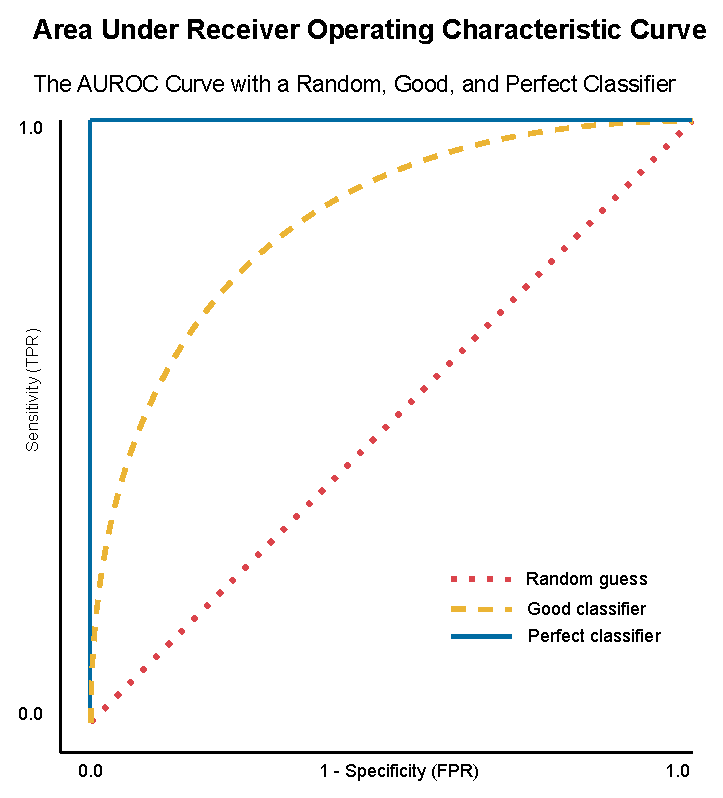
\includegraphics[width=0.45\textwidth]{images/auroc_goodie.drawio (3).pdf}
    \vspace{0.1em}
    \caption{{The AUROC Curve}}
    \subcaption*{The area under receiver operating characteristic curve is shown with a random guess, a good classifier, and a perfect classifier.}
    \label{fig:area-under-roc-curve-illustration}
\end{figure}

\subsubsection{Variable Importance Plot}

ML models have commonly been evaluated with only a single metric, such as accuracy \parencite{koalaverse-varimp}. However, it is increasingly important to not only focus on model predictions but also to understand how these predictions are made \parencite{doshi-velez-interpretable-machine-learning}. VIP shows the relative significance of each predictor variable in an ML model \parencite{koalaverse-varimp}, as shown in \autoref{fig:variable-importance-plot-theory}. VIP is calculated differently across ML models, but the core idea is to display the relative importance of predictor variables \parencite{wei-variable-importance-a-comorehensive-review}. VIP can be applied in R using the \texttt{vip::vip()} function \parencite{vip-documentation}. 

\begin{figure}[H]
    \centering
    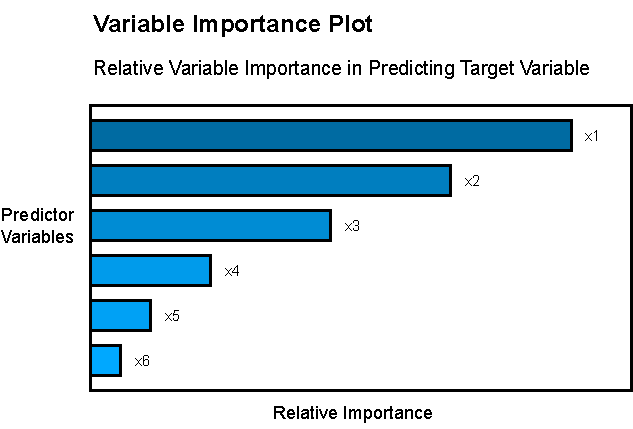
\includegraphics[width=0.6\textwidth]{images/variable-importance.drawio (3).pdf}
    \vspace{1em}
    \caption{{VIP}}
    \subcaption*{This shows the relative importance of predictor variables in predicting the target variable. Note that these are relative metrics, and absolute numbers will deviate between GLM and XGBoost models, as seen in \autoref{Results and discussion}.}
    \label{fig:variable-importance-plot-theory}
\end{figure}

\subsection{Summary of Methodology}

In this section, we first looked at ML and the application of ML methods in finance. We introduced the ML models GLM and XGBoost, where both will be used in the portfolio simulation in \autoref{Results and discussion}.  Further, we also introduced PPT, the conditional PPT, and the ML performance metrics, as summarised in \autoref{tab:methodology-performance-metrics}. For the numeric ranges in \autoref{tab:methodology-performance-metrics}, values closer to 1 are desirable. 

\begin{table}[H]
\centering
\begin{tabularx}{0.5\textwidth}{XX}
\hline
Metric       & Range \\
\hline
Accuracy              & [0, 1] \\
Precision             & [0, 1] \\
Sensitivity           & [0, 1] \\
Specificity           & [0, 1] \\
F-score               & [0, 1] \\
AUROC                 & [0.5, 1] \\
VIP & Relative \\
\hline
\end{tabularx}
\vspace{1em}
\caption{{Summary of ML Evaluation Metrics}}
\subcaption*{In principle we are looking for higher values for the performance metrics accuracy, precision, sensitivity, specificity, F-score, and AUROC. In \autoref{Results and discussion} we will discuss how only looking at accuracy measures may be misleading depending on the practical application of an ML model.}
\label{tab:methodology-performance-metrics}
\end{table}

